
\section{Architecture Integration}

\subsection{Model Support}

\begin{table}[H]
\centering
\small
\begin{tabular}{llllll}
\toprule
\textbf{Model} & \textbf{Attention class} & \textbf{Nested?} & \textbf{RoPE?} & \textbf{GQA?} & \textbf{Verified} \\
\midrule
DistilBERT & \texttt{MultiHeadSelfAttention} & No & No & No &  \\
RoBERTa & \texttt{BertSelfAttention} (nested) & Yes & No & No &  \\
GPT-2 & \texttt{GPT2Attention} (Conv1D) & No & No & No &  \\
Qwen3.5 & \texttt{Qwen3Attention} & No & Yes & Yes & 0.85 \\
\bottomrule
\end{tabular}
\end{table}

\subsection{Adaptive Rank}

Infini-Attention scales compression dimensions based on model depth:

\begin{lstlisting}
num\_layers = config.num\_hidden\_layers
if num\_layers \textgreater{} 12:
    self.rank = max(self.rank, 128)
    self.lora\_rank = max(self.lora\_rank, 32)
elif num\_layers \textgreater{} 6:
    self.rank = max(self.rank, 64)
    self.lora\_rank = max(self.lora\_rank, 32)
\end{lstlisting}

This ensures RoBERTa (12 layers) and larger models get sufficient 
capacity.

\subsection{Copy Weights}

\subsubsection{DistilBERT (Flat)}

\begin{lstlisting}
extracted["q"] = (src.q\_lin.weight.data, src.q\_lin.bias.data)
extracted["k"] = (src.k\_lin.weight.data, src.k\_lin.bias.data)
extracted["v"] = (src.v\_lin.weight.data, src.v\_lin.bias.data)
extracted["o"] = (src.out\_lin.weight.data, src.out\_lin.bias.data)
\end{lstlisting}

\texttt{is\_nested\_encoder = False}.

\subsubsection{RoBERTa (Nested)}

\begin{lstlisting}
s = src.self
extracted["q"] = (s.query.weight.data, s.query.bias.data)
extracted["k"] = (s.key.weight.data, s.key.bias.data)
extracted["v"] = (s.value.weight.data, s.value.bias.data)
extracted["o"] = (src.output.dense.weight.data, src.output.dense.bias.data)
\end{lstlisting}

\texttt{is\_nested\_encoder = True} (RoBERTa's \texttt{attention.output.dense} applies the 
output projection).

\subsubsection{GPT-2 (Conv1D)}

\begin{lstlisting}
w = src.c\_attn.weight.data.t()  # transpose
q\_w, k\_w, v\_w = w.chunk(3, dim=0)
extracted["q"] = (q\_w, src.c\_attn.bias.data[:768])
extracted["k"] = (k\_w, src.c\_attn.bias.data[768:1536])
extracted["v"] = (v\_w, src.c\_attn.bias.data[1536:2304])
extracted["o"] = (src.c\_proj.weight.data.t(), src.c\_proj.bias.data)
\end{lstlisting}

\subsubsection{Qwen (GQA + RoPE)}

Direct copy from \texttt{q\_proj/k\_proj/v\_proj/o\_proj}; RoPE preserved via 
\texttt{rotary\_emb}.

\subsection{Nested Encoder Detection}

\begin{lstlisting}
cls\_name = src.\_\_class\_\_.\_\_name\_\_
has\_out = (hasattr(src, "dense") or hasattr(src, "out\_proj")
           or hasattr(src, "out\_lin") or hasattr(src, "c\_proj")
           or hasattr(src, "o\_proj"))

is\_nested = False
if (cls\_name in ["BertSelfAttention", "RobertaSelfAttention", ...]
    or (hasattr(src, "query") and not has\_out)):
    is\_nested = True
if hasattr(src, "self") and hasattr(src, "output"):
    is\_nested = True
self.is\_nested\_encoder = is\_nested
\end{lstlisting}

\subsection{Injection}

\begin{lstlisting}
def inject\_infini(layer, model\_config=None, old\_attn=None, **kwargs):
    src = old\_attn or find\_attention(layer)
    new\_attn = InfiniAttention(config=model\_config, old\_attn=src, **kwargs)
    if src is not None:
        new\_attn.copy\_weights(src)
    replace\_attention(layer, new\_attn)
    return new\_attn
\end{lstlisting}

\subsection{The `InfiniAttention` Module Structure}

\begin{lstlisting}
class InfiniAttention(BaseAttention):
    def \_\_init\_\_(self, config, rank=64, compress\_dim=128,
                 local\_window=128, pretrained\_attn=None, ...):
        super().\_\_init\_\_(config, rank)
        self.q\_proj = LoRALinear(d, H*d\_h, lora\_rank=r)
        self.k\_proj = LoRALinear(d, H\_kv*d\_h, lora\_rank=r)
        self.v\_proj = LoRALinear(d, H\_kv*d\_h, lora\_rank=r)
        self.out\_proj = LoRALinear(H*d\_h, d, lora\_rank=r)
        
        self.memory = nn.Parameter(torch.randn(1, H, d\_c, d\_h) * 0.001)
        self.beta = nn.Parameter(torch.tensor([-5.0]))
        
        if pretrained\_attn is not None:
            self.copy\_weights(pretrained\_attn)
\end{lstlisting}

\subsection{Causality}

For decoders, the causal + window mask ensures:

\[
M\_{ij} = \begin{cases} 0 & j \leq i \text{ and } i - j \textless{} W \\ -\infty & \text{otherwise} \end{cases}
\tag{5.1}
\]

\textbf{Verification.} Gradient of output at position $i$ w.r.t. input at 
position $j > i$ is zero.

\subsection{Failure Modes}

\begin{table}[H]
\centering
\small
\begin{tabular}{lll}
\toprule
\textbf{Failure} & \textbf{Detection} & \textbf{Response} \\
\midrule
Missing projection & \texttt{copy\_weights} raises & Injection fails \\
Small Frobenius norm & Explicit check & Raises RuntimeError \\
Nested encoder mis-set & Logits differ & Manual fix \\
OOM & RuntimeError & Reduce batch \\
NaN in memory & \texttt{torch.isnan} & Not handled \\
\bottomrule
\end{tabular}
\end{table}

\subsection{Registry}

\begin{lstlisting}
@ATTENTION\_REGISTRY.register("infini")
@ATTENTION\_REGISTRY.register("infini\_attention")
class InfiniAttention(BaseAttention):
    ...
\end{lstlisting}

\subsection{Cross-Attention}

Infini-Attention \textbf{raises NotImplementedError} for cross-attention:

\begin{lstlisting}
if kwargs.get("encoder\_hidden\_states", None) is not None:
    raise NotImplementedError(...)
\end{lstlisting}

This is a limitation for encoder-decoder models.
\begin{lstlisting}

---
\end{lstlisting}

\begin{figure}[H]
\centering
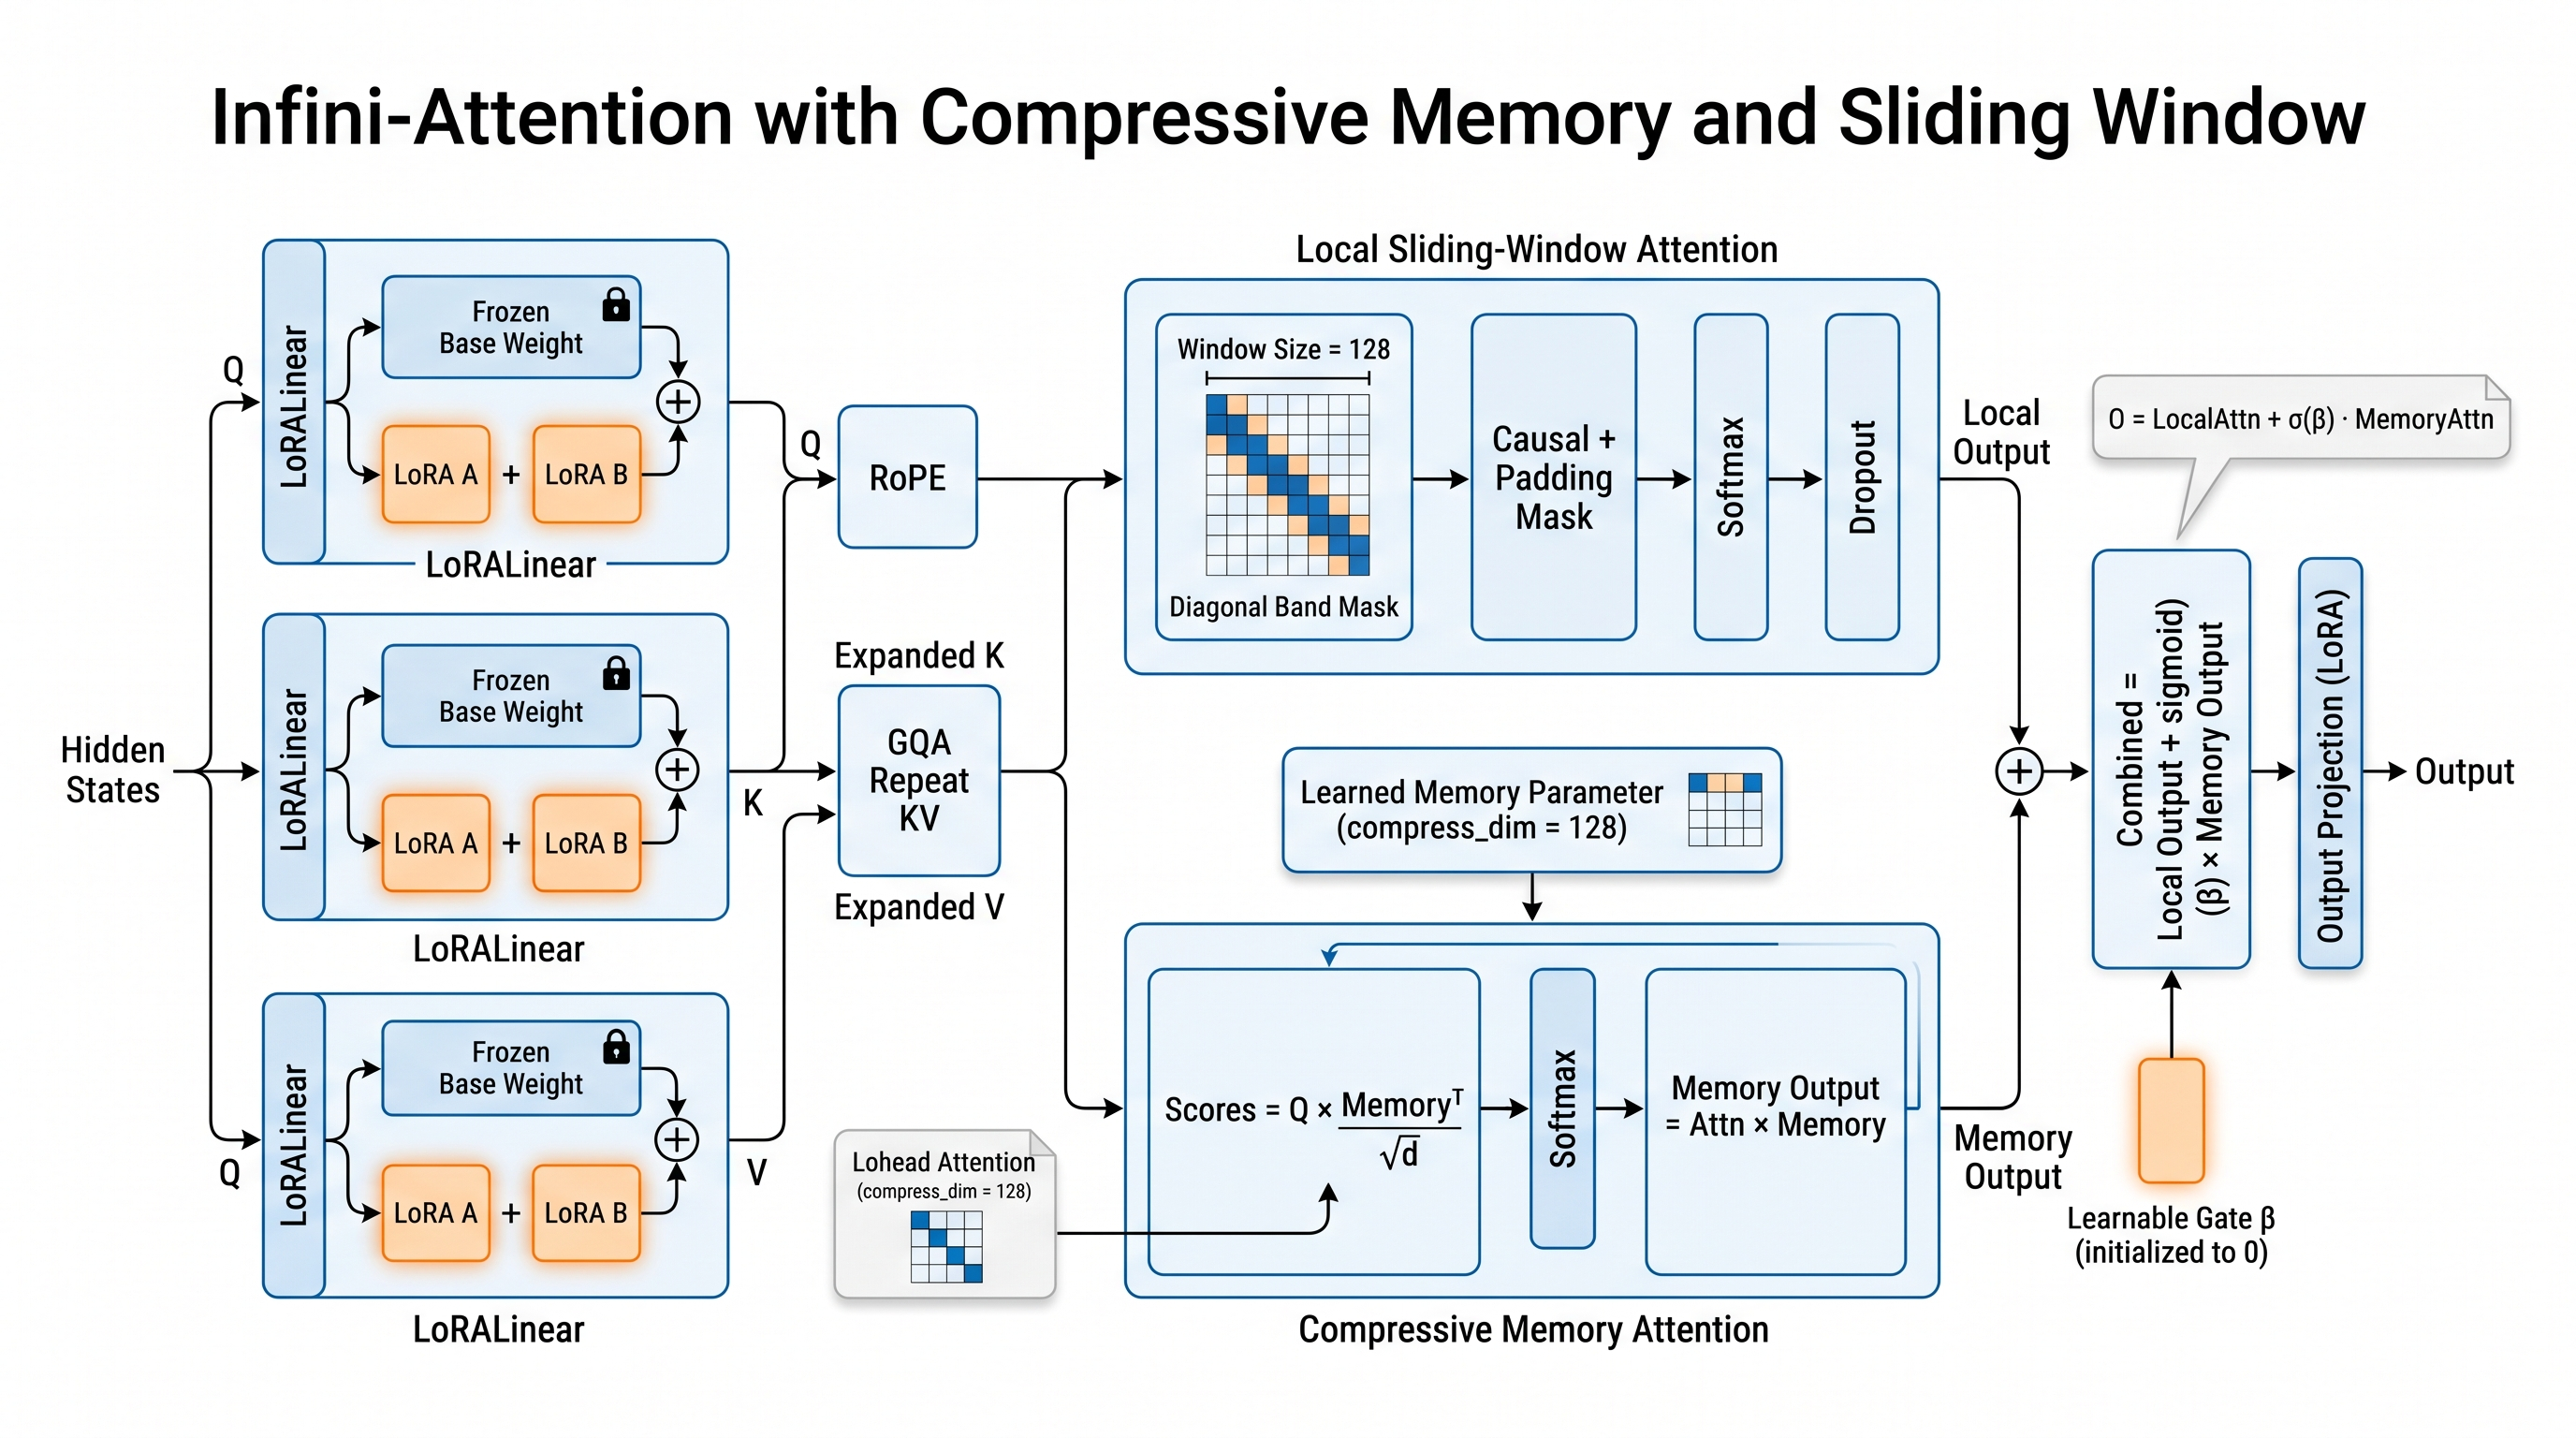
\includegraphics[width=\linewidth]{figures/architecture.jpeg}
\caption{High-level architectural diagram of infini.}
\label{fig:arch_infini}
\end{figure}

